\section{Dữ liệu}
\label{sec:du-lieu}

\subsection{Nguồn dữ liệu}
\label{sec:nguon-du-lieu}

Bộ dữ liệu sử dụng là Szeged Weather Dataset \cite{szegedweather}, ghi nhận quan trắc khí
tượng theo giờ tại thành phố Szeged, Hungary. File gốc có \textbf{96.453 dòng} và 12 cột:
\texttt{Formatted Date}, \texttt{Summary}, \texttt{Precip Type}, \texttt{Temperature (C)},
\texttt{Apparent Temperature (C)}, \texttt{Humidity}, \texttt{Wind Speed (km/h)},
\texttt{Wind Bearing (degrees)}, \texttt{Visibility (km)}, \texttt{Loud Cover},
\texttt{Pressure (millibars)}, \texttt{Daily Summary}. Khoảng thời gian trải từ
\textbf{2005-12-31 23:00} đến \textbf{2016-12-31 22:00} (thực chất là các năm
2006--2016, với một giờ cuối năm 2005 lọt vào do lệch múi giờ khi quy đổi mốc thời
gian gốc về UTC). Tần suất lấy mẫu gần như đều đặn theo giờ: sau khi sắp xếp theo thời
gian, có đúng 96.427 cặp bản ghi liên tiếp cách nhau 1 giờ, 24 cặp cách nhau 0 giờ (timestamp
trùng, xem Mục~\ref{sec:chat-luong-du-lieu}) và duy nhất 1 cặp cách nhau 4 giờ (một khoảng hở
thật sự trong dữ liệu gốc). Sau khi làm sạch và quy về lưới giờ liên tục
(Mục~\ref{sec:chat-luong-du-lieu}), bộ dữ liệu còn \textbf{96.432 dòng}, trong đó
\textbf{95.912 dòng có nhãn Rain/Snow hợp lệ}.

\subsection{Phân tích khám phá (EDA)}
\label{sec:eda}

\paragraph{Phân bố nhãn.} Trên 95.912 bản ghi có nhãn hợp lệ, \textbf{85.200 là Rain
(88,8\%)} và \textbf{10.712 là Snow (11,2\%)} -- bài toán mất cân bằng lớp rõ rệt
(tỷ lệ xấp xỉ 8:1), đúng như đã giả định khi thiết kế baseline lớp đa số
(Mục~\ref{sec:baseline}) và các chiến lược xử lý mất cân bằng (Mục~\ref{sec:mat-can-bang-lop-classic}).
Tỷ lệ Snow dao động theo năm từ 5,5\% (2014, năm ấm nhất trong giai đoạn khảo sát) đến
15,9\% (2011), không có xu hướng tăng/giảm đơn điệu rõ ràng (Hình~\ref{fig:eda-snow-year}).
Theo mùa, Snow gần như chỉ xuất hiện vào mùa Đông (37,9\% số giờ mùa Đông là Snow), rất
hiếm vào Xuân/Thu (3,9\% và 3,1\%), và \textbf{không một giờ nào trong mùa Hạ được gán
nhãn Snow} trong toàn bộ 11 năm dữ liệu (Hình~\ref{fig:eda-snow-season}).

\begin{figure}[H]
\centering
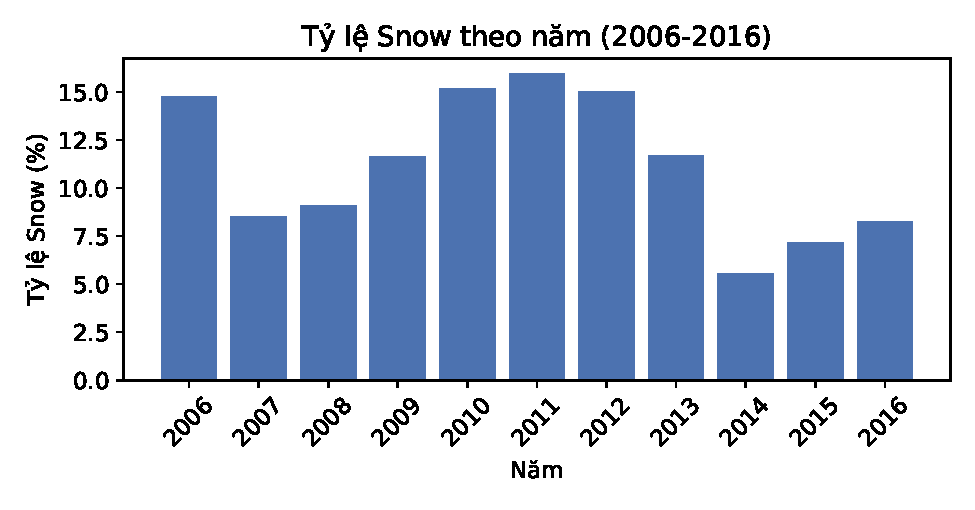
\includegraphics[width=0.78\textwidth]{figs/eda_snow_by_year.pdf}
\caption{Tỷ lệ Snow theo năm, 2006--2016.}
\label{fig:eda-snow-year}
\end{figure}

\begin{figure}[H]
\centering
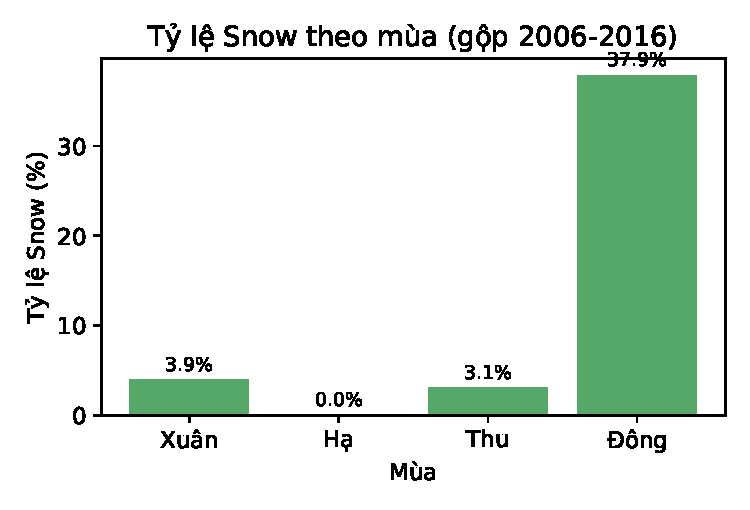
\includegraphics[width=0.62\textwidth]{figs/eda_snow_by_season.pdf}
\caption{Tỷ lệ Snow theo mùa, gộp toàn bộ 2006--2016.}
\label{fig:eda-snow-season}
\end{figure}

\paragraph{Phân bố nhiệt độ theo nhãn.} Hình~\ref{fig:eda-temp-label} vẽ phân bố nhiệt độ
của các bản ghi Rain và Snow. Phát hiện đáng chú ý: trên bộ dữ liệu này, \textbf{nhãn tách
gần như tuyệt đối theo dấu của nhiệt độ} -- toàn bộ 10.712 bản ghi Snow có nhiệt độ
$\le 0$\textdegree C (nhỏ nhất $-21{,}8$\textdegree C, lớn nhất đúng bằng
$0{,}0$\textdegree C), và toàn bộ 85.200 bản ghi Rain có nhiệt độ $> 0$\textdegree C (nhỏ
nhất $0{,}006$\textdegree C). Không tồn tại một bản ghi Rain nào ở nhiệt độ âm, cũng như
không có bản ghi Snow nào ở nhiệt độ dương. Quan sát này củng cố nghi vấn đã nêu ở
Mục~\ref{sec:han-che-nhan}: nhãn \texttt{Precip Type} của Dark Sky API nhiều khả năng cũng
được suy ra (một phần) từ chính ngưỡng nhiệt độ $0$\textdegree C khi có giáng thủy, chứ
không phải một quan trắc loại giáng thủy độc lập với nhiệt độ.

\begin{figure}[H]
\centering
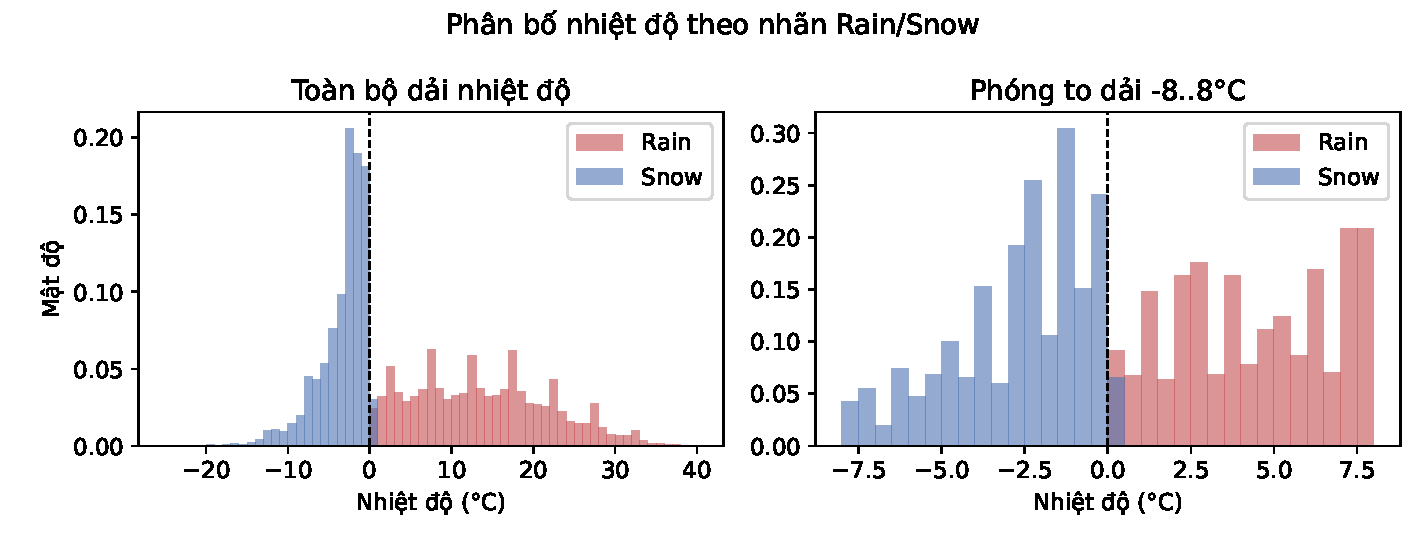
\includegraphics[width=0.95\textwidth]{figs/eda_temperature_by_label.pdf}
\caption{Phân bố nhiệt độ theo nhãn Rain/Snow -- toàn dải (trái) và phóng to quanh
ngưỡng $0$\textdegree C (phải). Đường nét đứt đánh dấu $0$\textdegree C.}
\label{fig:eda-temp-label}
\end{figure}

Vì vậy, cách gọi "\emph{vùng chồng lấn}" cần được hiểu chính xác hơn trên bộ dữ liệu này:
không phải hai lớp có giá trị nhiệt độ trùng nhau, mà là một \emph{dải gần ngưỡng} nơi phần
lớn các trường hợp Snow tập trung sát $0$\textdegree C thay vì rải đều ra các giá trị rất
âm. Cụ thể, trong dải $[-4, 4]$\textdegree C có 19.685 bản ghi, chiếm 38,4\% là Snow -- cao
hơn hẳn tỷ lệ nền 11,2\% -- cho thấy đây là dải nhiệt độ mà việc phân loại nhạy cảm nhất với
sai số hoặc giá trị thiếu của biến nhiệt độ. Nói cách khác: trên dữ liệu \emph{đầy đủ}, một
ngưỡng nhiệt độ đơn giản gần như giải quyết trọn vẹn bài toán (baseline ngưỡng nhiệt độ ở
Mục~\ref{sec:baseline} vì vậy được kỳ vọng rất mạnh khi không thiếu dữ liệu); nhưng khi
nhiệt độ bị thiếu theo kịch bản giả lập ở Mục~\ref{sec:gia-lap-mat-du-lieu} -- đặc biệt với
các bản ghi nằm trong dải sát ngưỡng này -- mô hình buộc phải dựa vào các biến tương quan
khác (độ ẩm, áp suất, gió) hoặc nội suy thay vì chỉ nhìn vào nhiệt độ, và đây chính là phần
việc khó thực sự mà đồ án muốn đánh giá.

\subsection{Hướng xử lý mất cân bằng dữ liệu}
\label{sec:xu-ly-mat-can-bang}

Tỷ lệ Rain:Snow xấp xỉ 8:1 (Mục~\ref{sec:eda}) khiến một mô hình không xử lý gì có thể đạt
Accuracy cao giả tạo (88,8\% chỉ bằng cách luôn đoán Rain) trong khi gần như không nhận ra
được Snow -- đúng là hành vi của baseline lớp đa số (Mục~\ref{sec:baseline}). Đồ án xử lý
vấn đề này ở \textbf{hai tầng độc lập}, áp dụng đồng thời:

\begin{enumerate}
  \item \textbf{Tầng đánh giá (không phụ thuộc thuật toán):} dùng \textbf{Macro F1} và
        \textbf{PR-AUC} làm chỉ số chính thay vì Accuracy (Mục~\ref{sec:metrics}) -- hai chỉ
        số này không bị "pha loãng" bởi lớp đa số, nên vẫn phản ánh đúng chất lượng kể cả
        khi không áp dụng bất kỳ kỹ thuật cân bằng nào ở bước huấn luyện.
  \item \textbf{Tầng thuật toán:} mỗi nhánh/baseline có cơ chế xử lý mất cân bằng riêng,
        phù hợp với bản chất mô hình (Bảng~\ref{tab:xu-ly-mat-can-bang}).
\end{enumerate}

\begin{table}[H]
\centering
\caption{Hướng xử lý mất cân bằng lớp theo từng thành phần.}
\label{tab:xu-ly-mat-can-bang}
\small
\begin{tabular}{@{}p{3.5cm}p{3.1cm}p{7.3cm}@{}}
\toprule
\textbf{Thành phần} & \textbf{Chiến lược} & \textbf{Cơ chế} \\
\midrule
Baseline Logistic Regression & \texttt{class\_weight}\newline\texttt{="balanced"} & Trọng số mỗi lớp tỷ lệ nghịch tần suất, áp trực tiếp vào hàm mất mát (\texttt{evaluation/baselines.py}). \\
\addlinespace
Baseline k-NN & Không xử lý & \texttt{KNeighborsClassifier} của scikit-learn không hỗ trợ trọng số lớp; giữ nguyên làm baseline "thô". \\
\addlinespace
Classic ML (XGBoost) & \texttt{scale\_pos\_weight}\newline (mặc định) hoặc SMOTE & \texttt{scale\_pos\_weight} = (số Rain)/(số Snow) trên tập train; SMOTE sinh thêm mẫu Snow tổng hợp trước khi huấn luyện (\texttt{models/classic.py}, \texttt{trainers/classic\_trainer.py}) -- so sánh hai chiến lược ở Mục~\ref{sec:ablation}. \\
\addlinespace
ROCKET (RidgeClassifierCV) & \texttt{class\_weight}\newline\texttt{="balanced"} & Trọng số nghịch tần suất lớp trong hàm mất mát ridge, đồng nhất với baseline Logistic Regression (\texttt{models/rocket.py}). \\
\addlinespace
Deep Learning\newline (mọi mô hình GRU/BRITS/SAITS) & Cross-entropy\newline có trọng số lớp & Trọng số lớp $c$ = $N / (2 \times \text{số mẫu lớp } c)$, áp cho cả vòng lặp huấn luyện tự cài lẫn \texttt{WeightedCrossEntropy} tuỳ biến cho PyPOTS (\texttt{trainers/deep\_trainer.py}). \\
\bottomrule
\end{tabular}
\end{table}

Baseline persistence và ngưỡng nhiệt độ không cần xử lý mất cân bằng: đây là các quy tắc
đơn giản (tra nhãn quá khứ, so sánh ngưỡng), không học qua một hàm mất mát nên khái niệm
"trọng số lớp" không áp dụng được. Với nhánh Classic ML, cả ba lựa chọn -- không xử lý,
\texttt{scale\_pos\_weight}, SMOTE -- đều được chạy và so sánh trực tiếp bằng Macro F1 ở
Mục~\ref{sec:ablation}, để trả lời câu hỏi kỹ thuật cân bằng nào thực sự cải thiện kết quả
trên bộ dữ liệu này thay vì mặc định chọn một chiến lược.

\subsection{Vấn đề chất lượng dữ liệu}
\label{sec:chat-luong-du-lieu}

Quá trình khảo sát dữ liệu phát hiện bốn vấn đề chất lượng cần xử lý trước khi huấn
luyện, đều được xử lý tự động trong \texttt{datasets/szeged.py:clean()}:

\begin{itemize}
  \item \textbf{Áp suất bằng 0:} \textbf{1.288 dòng} (1,3\% tổng số dòng gốc) có
        \texttt{Pressure~(millibars)~=~0} -- giá trị phi vật lý (áp suất khí quyển không
        thể bằng 0), được xem như giá trị thiếu và chuyển thành NaN.
  \item \textbf{Timestamp trùng:} \textbf{24 dòng} có mốc thời gian trùng với dòng ngay
        trước đó; bản ghi trùng bị loại, chỉ giữ bản ghi xuất hiện đầu tiên.
  \item \textbf{Cột hằng số:} cột \texttt{Loud Cover} chỉ nhận đúng một giá trị (0) trong
        toàn bộ 96.453 dòng, không mang thông tin phân biệt, nên bị loại khỏi tập đặc
        trưng đầu vào.
  \item \textbf{Nhãn bị thiếu:} \textbf{517 dòng} (0,5\%) có \texttt{Precip Type} rỗng
        hoặc khác \texttt{rain}/\texttt{snow}; các dòng này bị loại khỏi tập có nhãn hợp lệ
        nhưng \emph{vẫn được giữ lại} trong lưới giờ liên tục (giá trị đặc trưng của chúng
        vẫn dùng được làm ngữ cảnh lịch sử cho các cửa sổ khác, chỉ riêng nhãn bị đánh dấu
        thiếu) -- xem thêm Mục~\ref{sec:phat-bieu-bai-toan} về cách cửa sổ bị loại nếu nhãn
        tại $t+1$ không hợp lệ.
\end{itemize}

Ngoài ra, sau khi quy dữ liệu về lưới giờ liên tục theo từng giờ, phát hiện thêm
\textbf{520 giờ bị hở hoàn toàn} (không có bản ghi gốc nào, chủ yếu trùng với các dòng vừa
bị loại ở trên) -- đây là phần \emph{thiếu dữ liệu tự nhiên} của bộ dữ liệu, độc lập và được
giữ tách biệt với phần mất dữ liệu \emph{giả lập} dùng để đánh giá độ bền vững của mô hình ở
Mục~\ref{sec:gia-lap-mat-du-lieu}.

\subsection{Quy trình tiền xử lý}
\label{sec:quy-trinh-tien-xu-ly}

Toàn bộ quy trình từ CSV thô đến dữ liệu sẵn sàng huấn luyện gồm bốn bước tự động, lần
lượt nằm trong \texttt{datasets/szeged.py}, \texttt{datasets/windows.py} và
\texttt{datasets/splits.py} (Hình~\ref{fig:pipeline-tien-xu-ly}): \textbf{(1)} đọc và sắp
xếp dữ liệu thô theo thời gian; \textbf{(2)} làm sạch (loại cột hằng số, sửa giá trị phi
vật lý, loại bản ghi trùng/nhãn không hợp lệ, quy về lưới giờ liên tục -- chi tiết ở
Mục~\ref{sec:chat-luong-du-lieu}); \textbf{(3)} cắt cửa sổ trượt 24 giờ, gán nhãn tại giờ
$t{+}1$ ngay sau mỗi cửa sổ; \textbf{(4)} chia tập train/validation/test theo năm.

\begin{figure}[H]
\centering
\resizebox{0.78\textwidth}{!}{%
\begin{tikzpicture}[
  data/.style={rectangle, rounded corners, draw=black, fill=orange!15,
               minimum width=7.2cm, minimum height=1.0cm, align=center, font=\small},
  proc/.style={rectangle, draw=black, fill=blue!15,
               minimum width=7.2cm, minimum height=1.3cm, align=center, font=\small},
  split/.style={rectangle, rounded corners, draw=black, fill=orange!15,
                minimum width=2.2cm, minimum height=1.0cm, align=center, font=\small},
  arr/.style={thick, ->, >=stealth}
]
  \node[data] (csv) {CSV thô\\96.453 dòng $\times$ 12 cột};
  \node[proc, below=0.5cm of csv] (load) {\texttt{load\_raw()}\\Parse timestamp (UTC, naive), sắp xếp theo thời gian};
  \node[proc, below=0.5cm of load] (clean) {\texttt{clean()}\\Loại \texttt{Loud Cover} $\cdot$ Pressure=0$\to$NaN $\cdot$ dedupe\\ $\cdot$ lọc nhãn không hợp lệ $\cdot$ reindex lưới giờ liên tục};
  \node[data, below=0.5cm of clean] (cleaned) {DataFrame sạch: 96.432 dòng (lưới giờ liên tục)\\95.912 dòng có nhãn Rain/Snow hợp lệ};
  \node[proc, below=0.5cm of cleaned, minimum height=1.0cm] (window) {\texttt{build\_windows(window=24)}\\Cửa sổ trượt 24 giờ $\to$ nhãn tại $t{+}1$};
  \node[data, below=0.5cm of window] (windowed) {$X$: (95.888, 24, 5) $\quad$ $y$: (95.888,)};
  \node[proc, below=0.5cm of windowed, minimum height=1.0cm] (split) {\texttt{year\_split()}\\Chia theo năm, chống rò rỉ dữ liệu};
  \node[split, below=0.6cm of split, xshift=-2.6cm] (train) {Train\\69.962};
  \node[split, below=0.6cm of split] (val) {Val\\8.757};
  \node[split, below=0.6cm of split, xshift=2.6cm] (test) {Test\\17.169};

  \draw[arr] (csv) -- (load);
  \draw[arr] (load) -- (clean);
  \draw[arr] (clean) -- (cleaned);
  \draw[arr] (cleaned) -- (window);
  \draw[arr] (window) -- (windowed);
  \draw[arr] (windowed) -- (split);
  \draw[arr] (split) -- (train);
  \draw[arr] (split) -- (val);
  \draw[arr] (split) -- (test);
\end{tikzpicture}}
\caption{Quy trình tiền xử lý: từ CSV thô đến ba tập train/validation/test.}
\label{fig:pipeline-tien-xu-ly}
\end{figure}

Hai bước (3) và (4) chưa được mô tả ở Mục~\ref{sec:chat-luong-du-lieu}:

\begin{itemize}
  \item \textbf{Cắt cửa sổ trượt (\texttt{build\_windows}):} với mỗi vị trí $i$ trên lưới
        giờ liên tục, đặc trưng là 24 giờ $[i-23, i]$, nhãn là giá trị tại giờ $i+1$.
        Cửa sổ bị loại nếu nhãn tại $i+1$ không hợp lệ (NaN); \textbf{đặc trưng vẫn được
        giữ} dù một vài giờ trong cửa sổ trùng với phần thiếu dữ liệu tự nhiên
        (Mục~\ref{sec:chat-luong-du-lieu}) -- đây là lựa chọn có chủ đích, để phần thiếu
        tự nhiên (rất nhỏ, 0,42\% tổng số điểm) không bị trộn lẫn với phần mất dữ liệu
        \emph{giả lập} sẽ thêm vào ở Mục~\ref{sec:gia-lap-mat-du-lieu}.
  \item \textbf{Chia tập (\texttt{year\_split}):} chia theo \emph{thời gian}, không xáo
        trộn ngẫu nhiên -- train gồm các cửa sổ có nhãn thuộc 2006--2013, validation thuộc
        2014, test thuộc 2015--2016 (cố định, không dùng để chọn mô hình/siêu tham số).
        Cách chia này mô phỏng đúng kịch bản dự báo thực tế (dự đoán tương lai từ quá khứ)
        và tránh rò rỉ dữ liệu giữa các tập.
\end{itemize}

\subsection{Dữ liệu sau tiền xử lý}
\label{sec:du-lieu-sau-tien-xu-ly}

Sau bốn bước trên, dữ liệu sẵn sàng cho mọi nhánh phương pháp (Chương~\ref{sec:phuong-phap-de-xuat})
là hai mảng NumPy: $X$ kiểu \texttt{float32}, shape $(95{.}888,\ 24,\ 5)$ -- tương ứng
95.888 cửa sổ, mỗi cửa sổ 24 giờ $\times$ 5 biến (Mục~\ref{sec:nguon-du-lieu}) -- và $y$
kiểu \texttt{int64}, shape $(95{.}888,)$ với $y \in \{0 \text{ (Rain)}, 1 \text{ (Snow)}\}$.
Tỷ lệ Snow trong $y$ là 11,2\%, khớp với tỷ lệ trên toàn bộ dữ liệu có nhãn
(Mục~\ref{sec:eda}) -- việc cắt cửa sổ không làm lệch phân bố lớp. $X$ còn chứa NaN tại
0,42\% số điểm, đúng bằng phần thiếu dữ liệu tự nhiên đã nêu ở
Mục~\ref{sec:chat-luong-du-lieu} (chưa tính phần giả lập thêm ở Chương~\ref{sec:phuong-phap-de-xuat}).
Ba tập được đánh chỉ số (không sao chép dữ liệu) theo Mục~\ref{sec:quy-trinh-tien-xu-ly}:
69.962 cửa sổ train, 8.757 validation, 17.169 test.

Bảng~\ref{tab:vi-du-cua-so} minh hoạ cụ thể một cửa sổ thật (cửa sổ đầu tiên của tập
train): 24 giờ từ 31/12/2005 23:00 đến 01/01/2006 22:00 là đặc trưng đầu vào, nhãn
Rain được lấy từ giờ \textbf{01/01/2006 23:00} -- đúng là giờ ngay sau cửa sổ, không phải
giờ cuối cùng của cửa sổ.

\begin{table}[H]
\centering
\caption{Ví dụ một cửa sổ đầu vào thật (rút gọn, chỉ hiện 3 giờ đầu và 3 giờ cuối trong 24 giờ).}
\label{tab:vi-du-cua-so}
\small
\begin{tabular}{@{}lccccc@{}}
\toprule
Giờ & Temp. (°C) & Humidity & Wind (km/h) & Pressure (mb) & Visib. (km) \\
\midrule
31/12 23:00 & 0,58 & 0,89 & 17,11 & 1016,66 & 9,98 \\
01/01 00:00 & 1,16 & 0,85 & 16,62 & 1016,15 & 9,90 \\
01/01 01:00 & 1,67 & 0,82 & 20,25 & 1015,87 & 9,90 \\
\multicolumn{6}{c}{$\vdots$ (18 giờ còn lại)} \\
01/01 20:00 & 4,93 & 0,86 & 23,94 & 1009,43 & 15,73 \\
01/01 21:00 & 5,47 & 0,87 & 22,72 & 1009,51 & 14,80 \\
01/01 22:00 & 5,42 & 0,86 & 19,56 & 1009,64 & 15,65 \\
\bottomrule
\end{tabular}

\vspace{2pt}
\footnotesize Nhãn tại $t{+}1$ = 01/01 \textbf{23:00} $\to$ \textbf{Rain} ($y=0$).
\end{table}

\subsection{Sinh mặt nạ thiếu dữ liệu giả lập}
\label{sec:sinh-mat-na}

Phần thiếu dữ liệu \emph{tự nhiên} của bộ dữ liệu rất nhỏ (0,42\% số điểm,
Mục~\ref{sec:du-lieu-sau-tien-xu-ly}) -- không đủ để đánh giá mô hình hoạt động tốt đến
đâu khi cảm biến thực sự mất số đo. Vì vậy, ngay trên $X$ đã tiền xử lý, đồ án \textbf{giả
lập thêm} mất dữ liệu theo ba kiểu, ở ba tỷ lệ 10/30/50\% (mô tả đầy đủ về động cơ và thiết
kế ở Mục~\ref{sec:gia-lap-mat-du-lieu}; phần này trình bày cụ thể mặt nạ được sinh ra như
thế nào và trông như thế nào trên dữ liệu thật):

\begin{itemize}
  \item \textbf{Point:} từng điểm $(giờ, biến)$ bị ẩn độc lập, chọn ngẫu nhiên không lặp
        trong số các điểm đang quan sát được -- mô phỏng nhiễu đo/lỗi gói tin rời rạc.
  \item \textbf{Subsequence:} nhiều đoạn liên tiếp ngắn/vừa (độ dài ngẫu nhiên, tối đa nửa
        cửa sổ), mỗi đoạn trên \emph{một} biến -- mô phỏng mất kết nối tạm thời.
  \item \textbf{Block:} một hoặc nhiều biến bị ẩn \emph{toàn bộ} trong một đoạn thời gian
        dài (tối thiểu nửa cửa sổ) -- mô phỏng một cảm biến hỏng hẳn trong thời gian dài.
\end{itemize}

Với mỗi cửa sổ, \texttt{datasets/missingness.py:generate\_mask()} tính trước một
\emph{ngân sách} = (tỷ lệ mục tiêu $\times$ 120 điểm/cửa sổ) $-$ (số điểm đã thiếu tự
nhiên), rồi chọn đúng số điểm đó để ẩn thêm theo kiểu tương ứng -- nhờ vậy tỷ lệ thiếu
\emph{thực tế} luôn sát tỷ lệ mục tiêu dù dữ liệu vốn đã có một ít NaN tự nhiên
(Bảng~\ref{tab:ty-le-mat-du-lieu-thuc-te}). Mặt nạ được sinh với \textbf{seed cố định}
một lần duy nhất và lưu cache (\texttt{outputs/masks/}), để cả ba nhánh phương pháp dùng
chung đúng một mặt nạ cho mỗi cấu hình -- điều kiện bắt buộc để so sánh công bằng.

\begin{figure}[H]
\centering
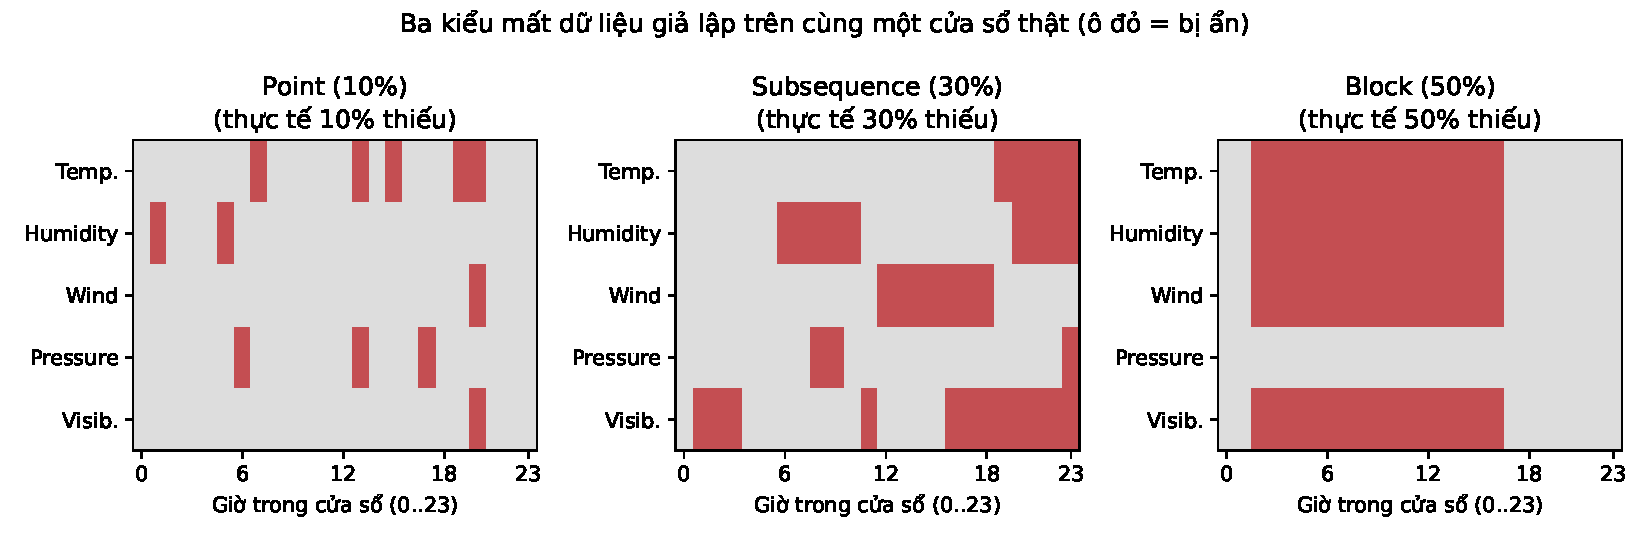
\includegraphics[width=0.95\textwidth]{figs/missingness_mask_example.pdf}
\caption{Ba kiểu mất dữ liệu giả lập áp lên \emph{cùng một} cửa sổ 24 giờ $\times$ 5 biến
thật (không có NaN tự nhiên để mặt nạ hiện rõ): point rải rác từng điểm, subsequence tạo
đoạn liên tiếp trên từng biến, block xoá nguyên biến trong một khoảng thời gian dài.}
\label{fig:missingness-example}
\end{figure}

\begin{table}[H]
\centering
\caption{Tỷ lệ thiếu mục tiêu so với thực tế, đo trên toàn bộ 95.888 cửa sổ (seed=123).}
\label{tab:ty-le-mat-du-lieu-thuc-te}
\small
\begin{tabular}{@{}lccc@{}}
\toprule
\textbf{Kiểu} & \textbf{Mục tiêu 10\%} & \textbf{Mục tiêu 30\%} & \textbf{Mục tiêu 50\%} \\
\midrule
Point & 10,14\% & 30,06\% & 50,02\% \\
Subsequence & 10,14\% & 30,06\% & 50,02\% \\
Block & 10,14\% & 30,06\% & 50,02\% \\
\bottomrule
\end{tabular}
\end{table}

Sai lệch nhỏ và đều giữa ba kiểu (ví dụ 10,14\% thay vì đúng 10,00\%) đến từ việc làm tròn
ngân sách về số nguyên trên từng cửa sổ 120 điểm, cộng thêm 0,42\% đã thiếu sẵn tự nhiên --
không phải do lỗi thuật toán, và sai lệch này giống hệt nhau ở cả ba kiểu vì cùng dùng
chung một công thức ngân sách.

\subsection{Hạn chế của nhãn}
\label{sec:han-che-nhan}

Nhãn Rain/Snow trong bộ dữ liệu Szeged không phải là kết quả quan trắc trực tiếp từ trạm
khí tượng, mà được sinh ra từ dịch vụ Dark Sky API dựa trên mô hình nội suy/dự báo của
bên thứ ba. Phát hiện ở Mục~\ref{sec:eda} -- nhãn tách gần như tuyệt đối theo dấu của
nhiệt độ, không có một ngoại lệ nào trong hơn 95 nghìn bản ghi -- củng cố khả năng nhãn này
\emph{chính nó} đã được suy ra (một phần) từ nhiệt độ bằng một quy tắc tương tự, chứ không
phải một quan trắc loại giáng thủy độc lập. Do đó, mọi so sánh hiệu năng giữa các phương
pháp trong báo cáo này cần được hiểu là so sánh dựa trên nhãn suy ra từ Dark Sky, không
phải nhãn quan trắc thực địa tuyệt đối; một mô hình "học được đúng ngưỡng nhiệt độ" có thể
đơn giản là đang học lại chính quy tắc đã sinh ra nhãn, chứ chưa chắc phản ánh khả năng
phân biệt Rain/Snow trong các tình huống phức tạp hơn (ví dụ mưa đóng băng, mưa tuyết hỗn
hợp) mà quy tắc đơn giản này không có bản ghi nào để phân biệt. Hạn chế này được thảo luận
lại ở Mục~\ref{sec:han-che}.
